\subsection{Classifiers}

\subsubsection{Logistic Regression}
Logistic regression is a statistical model used for binary classification problems. It predicts the probability of a binary outcome based on one or more predictor variables. Unlike linear regression, which predicts a continuous value, logistic regression predicts the probability that a given instance belongs to a particular class.

The logistic function, also known as the sigmoid function, is the cornerstone of logistic regression. It transforms any real-valued number into a value between 0 and 1. The logistic function is defined as:

\begin{equation}
    \sigma(z) = \frac{1}{1 + e^{-z}}
\end{equation}

where \(z\) is a linear combination of the predictor variables:

\begin{equation}
    z = b_0 + b_1x_1 + b_2x_2 + \ldots + b_nx_n
\end{equation}

Here, \(b_0\) is the intercept term, \(b_i\) are the coefficients, and \(x_i\) are the predictor variables.\\

The logistic function outputs probabilities, which can be interpreted as the likelihood of an instance belonging to a particular category. The odds of an event is defined as the ratio of the probability of the event occurring to the probability of it not occurring:

\begin{equation}
    \text{Odds} = \frac{p}{1-p}
\end{equation}

The likelihood function in logistic regression measures how well the model predicts the target variable. It is defined as:

\begin{equation}
    L(b_0, b_1, \ldots, b_n) = \prod_{i=1}^{m} P(y_i|x_i)
\end{equation}

where \(m\) is the number of samples in the dataset for which the prediction is made, \(y_i\) is the actual class label of the \(i\)-th instance, and \(P(y_i|x_i)\) is the predicted probability of \(y_i\) given \(x_i\).\\


In logistic regression, the goal is to maximize the likelihood function, which is equivalent to minimizing the negative log-likelihood, known as the cross-entropy loss:

\begin{equation}
    \mathcal{L}(b_0, b_1, \ldots, b_n) = -\frac{1}{m}\sum_{i=1}^{m} \left[y_i\log\left(P(y_i=1|x_i)\right) + (1-y_i)\log\left(1-P(y_i=1|x_i)\right)\right]
\end{equation}


To find the optimal coefficients, iterative optimization algorithms like gradient descent or Newton's method are used. These methods adjust the coefficients to minimize the loss function.

\subsubsection{Decision Tree}

Decision trees are versatile machine learning models used for both classification and regression tasks. A decision tree is a hierarchical structure composed of nodes. The top node is called the \textit{root}, and the final nodes are \textit{leaves}. Internal nodes represent features, and edges represent decisions.

\begin{figure}[h]
    \centering
    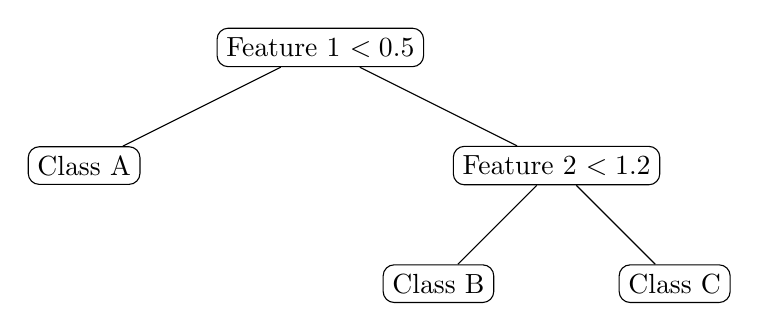
\begin{tikzpicture}[
        level/.style={sibling distance=60mm/#1},
        every node/.style = {shape=rectangle, rounded corners,
          draw, align=center,
          top color=white, bottom color=white}
        ]
        \node {Feature 1 $< 0.5$}
            child { node {Class A}
            }
            child { node {Feature 2 $< 1.2$}
                child { node {Class B}
                }
                child { node {Class C}
                }
            };
    \end{tikzpicture}
    \caption{Example Decision Tree Structure}
\end{figure}


At each node, the decision tree algorithm selects the best feature to split the data based on a certain criterion. Common criteria include Gini impurity and entropy.

The Gini impurity for a node \(m\) containing instances of class \(k\) is calculated as:

\begin{equation}
    Gini(m) = 1 - \sum_{k=1}^{n} (p_{mk})^2
\end{equation}

where \(n\) is the number of classes and \(p_{mk}\) is the probability of an instance in node \(m\) belonging to class \(k\).

Entropy measures the impurity or disorder of a set of instances. For a node \(m\), the entropy is given by:

\begin{equation}
    H(m) = -\sum_{k=1}^{n} p_{mk} \log(p_{mk})
\end{equation}

The decision tree algorithm recursively splits the data until a stopping criterion is met (e.g., a maximum depth is reached or a minimum number of samples per leaf is attained).

To make predictions, an instance is passed through the tree starting at the root. At each node, a decision based on a feature is made, and the instance is directed to the corresponding child node. This process continues until a leaf node is reached, and the predicted outcome is associated with that leaf.

\subsubsection{Random Forest}

Random Forest is an ensemble learning method used for both classification and regression tasks. The main idea of ensemble learning is combining the predictions from multiple models to get better predictive performance. Random forest operates by constructing a multitude of decision trees at training time and outputting the class (classification) or mean prediction (regression) of the individual trees.\\

Another import concept is bagging, which involves creating multiple datasets by sampling with replacement from the original data. Each dataset is used to train a base learner. In Random Forest, each tree is constructed using a different bootstrap sample.\\

 Random Forest is an example of a bagging ensemble method, where each base learner (decision tree) is trained on a random subset of the data.\\


In addition to using random subsets of the data, Random Forest also uses random subsets of features at each split. This helps to decorrelate the trees, making the ensemble more robust.\\

Each tree in a Random Forest is grown to its maximum depth, or until it reaches a minimum number of samples per leaf. This allows individual trees to capture complex relationships in the data.\\

For classification tasks, the final prediction is determined by a majority vote among the trees. For regression tasks, the final prediction is the average of the predictions from all trees.

\subsubsection{XGBoost}


XGBoost (Extreme Gradient Boosting), is an ensemble learning algorithm known for its efficiency and accuracy in a wide range of machine learning tasks. It is based on the gradient boosting, which combines the predictions of multiple weak learners (typically decision trees) to produce a strong learner. \\

Gradient boosting is a machine learning technique that builds an additive model in a forward stage-wise manner. It starts with an initial weak model and then iteratively improves it by fitting new models to the residual errors of the previous models. \\

The final prediction is obtained by summing the predictions of all the models. In XGBoost, the weak learners are decision trees. These trees are shallow, meaning they have a limited depth, which helps in reducing overfitting. The training process involves finding the best splits at each node to minimize the loss function.


\end{document}



